\chapter{Lecture 20 - Fourier-Legendre Series Expansion}
\label{ch:lec20}
\section{Objectives}
\begin{itemize}
\item Recap the Legendre equation as a Sturm-Liouville problem and give its orthogonality relation.
\item Give an example to show the expansion of a function in terms of Legendre polynomials.
\end{itemize}
\setcounter{lstannotation}{0} %hack to try and re-set annotation counter.
\section{Orthogonality with Legendre Polynomials}
We have some experience with Legendre's equation and their solutions Legendre polynomials.  As a recap, however, Legendre's equation is shown in Equation \ref{eq:lec20-legendre-eq}.
\begin{equation}
\left(1-x^2\right)u^{\prime \prime} - 2xu^{\prime} + n(n+1)u = 0, \ \ x \in (-1,1)
\label{eq:lec20-legendre-eq}
\end{equation}
The general solution is $u(x) = c_nP_n(x)$ where $P_n(x)$ is the Legendre polynomial of order $n$.\marginnote{As a reminder the first few Legendre polynomials are: $P_0(x) = 1$, $P_1(x) = x$, $P_2(x) = \frac{1}{2}\left(3x^2-1\right)$, and $P_3(x) = \frac{1}{2}\left(5x^3-3x\right)$.}  

As demonstrated in Lecture 18, the self-adjoint form for Legendre's equation is given in Equation \ref{eq:lec20-legendre-sa}.
\begin{equation}
\frac{d}{dx}\left[\left(1-x^2 \right) u^{\prime} \right] + \overbrace{n(n+1)}^{\lambda}u = 0
\label{eq:lec20-legendre-sa}
\end{equation}
The orthogonality relation is shown below:\marginnote[1.0cm]{Recall that for Legendre's equation, the weight function $p(x)$ is equal to 1. Also recall that $\left(P_n,P_n \right) = \sfrac{2}{2n+1}$.}
\begin{equation*}
\int_{-1}^{1} P_m(x)P_n(x) (1) \ dx = 
\begin{cases}
0, & m\ne n \\
\frac{2}{2n+1}, & m=n
\end{cases}
\end{equation*}
If we need to represent a function $f(x)$ in terms of Legendre polynomials, we can carry out a \emph{Fourier-Legendre} expansion as shown below:\marginnote[1.0cm]{As usual we can derive the formulas for the coefficients $c_n$ of Equation \ref{eq:lec20-FL-coeff} by multiplying both sides of Equation \ref{eq:lec20-FL-exp} by $P_n(x)$ and integrating.}
\begin{align}
f(x) &= \sum\limits_{n=0}^{\infty}c_n P_n(x) \label{eq:lec20-FL-exp}\\ 
\text{where:}& \nonumber \\
c_n &= \frac{\left(f(x),P_n(x) \right)}{\left(P_n(x),P_n(x) \right)} = \frac{\int_{-1}^{1} f(x) P_n(x) \ dx}{\sfrac{2}{2n+1}} 
\label{eq:lec20-FL-coeff}
\end{align}

The convergence of Fourier-Legendre series expansions behave similarly to the Fourier series expansion using trigonometric polynomials.  This behavior is recapitulated in the next theorem.\marginnote[1.0cm]{This also happens to be true for Fourier-Bessel expansions.} 

\begin{theorem}[Convergence of Fourier-Legendre Series]
Let $f(x)$ and $f^{\prime}(x)$ be piece-wise continuous on the interval $[-1,1]$. Then for all $x$ in the interval, the Fourier-Legendre series of $f$ converges to $f(x)$ at a point where $f(x)$ is continuous and to the average:
\begin{equation*}
\frac{f(x^+) + f(x^-) }{2}
\end{equation*}
at points where $f(x)$ is discontinuous.
\end{theorem}

\vspace{0.5cm}

\noindent\textbf{Example:} Construct the Fourier-Legendre expansion of:
\begin{equation*}
f(x) = 
\begin{cases}
0, & -1 < x < 0 \\
1, & 0 \le x < 1
\end{cases}
\end{equation*}

Since the tools we need to use have largely be introduced already, I will simply present the necessary MATLAB code in a single listing.
\marginnote[2.5cm]{
\ref{lst:ann20-1} Recall that $P_0(x) = 1$ and, according to our formula, 
\begin{align*}
\left(P_0(x),P_0(x)\right) &= \frac{2}{2n+1} \\
  &= \frac{2}{2(0)+1} \\
  &= 2.
\end{align*}
Hence:
\begin{align*}
c_0 &= \frac{\left(f(x),P_0\right)}{\left(P_0,P_0\right)} \\
&= \frac{\int_{-1}^1 f(x) (1) \ dx}{2}
\end{align*}
}
\marginnote[0.5cm]{
\ref{lst:ann20-2} In addition to using the formula for $\left(P_n(x),P_n(x)\right)$ we use the built-in MATLAB function for constructing $P_n(x)$: \lstinline[style=myMatlab]{legendreP(n,x)}.
}
\begin{lstlisting}[name=lec20_ex, style=myMatlab]
clear
clc
close 'all'

f = @(x) ex1(x);

N = 15; % number of terms 
a = -1; b = 1; % boundaries

% handle Po coefficient separately
c0 = (1/2)*integral(@(x) f(x),a,b);  /*!\annotation{lst:ann20-1}!*/
cn = nan(N-1,1);
error_norm = nan(N,1); 

FL = @(x) c0;

% calculate relative error
err_fn = @(x) FL(x) - f(x);
error_norm(1) = integral(@(x) err_fn(x).^2,a,b)./...
        integral(@(x) f(x).^2,a,b); 

for n = 1:(N-1)
    % compute the n'th coefficient /*!\annotation{lst:ann20-2}!*/
    cn(n) = ((2*n+1)/2)*integral(@(x) f(x).*legendreP(n,x),a,b); 
    FL = @(x) FL(x) + cn(n)*legendreP(n,x); %update the expansion
    
    % compute the error.
    err_fn = @(x) FL(x) - f(x);
    error_norm(n+1) = integral(@(x) err_fn(x).^2,a,b)./...
        integral(@(x) f(x).^2,a,b); % normalize error by size of function.
end

%% Plot the result
Nx = 1000;
X = linspace(a,b,Nx);

figure(1)
plot(X,FL(X),'-g',...
    X,f(X),'--b',...
    'LineWidth',3);
grid on
xlabel('X','fontsize',14,'fontweight','bold');
ylabel('f(X)','fontsize',14,'fontweight','bold');
titlestr = ...
    sprintf('Fourier-Legendre expansion, N = %d',N);
title(titlestr,'fontsize',16,'fontweight','bold');
set(gca,'fontsize',12,'fontweight','bold');

%% Plot the error
figure(2)
loglog(1:N,error_norm,'-ok','linewidth',3);
title('Convergence behavior','fontsize',16,'fontweight','bold');
grid on
xlabel('Number of Fourier-Legendre Terms','fontsize',14,'fontweight','bold');
ylabel('Relative Error','fontsize',14,'fontweight','bold');
set(gca,'fontsize',12,'fontweight','bold');


%% Local functions
function y = ex1(x)
[m,n] = size(x); 
% expect vector inputs.
assert(min(m,n) == 1,'Bad input for ex1');  /*!\annotation{lst:ann20-3}!*/
% construct y so that it has the same shape as x
y = nan(m,n); 
for i = 1:length(x) 
    if (x(i) > -1) && (x(i) < 0) 
        y(i) = 0;
    elseif (x(i) >= 0) && (x(i) < 1)
        y(i) = 1;
    end
end
end
\end{lstlisting}
\marginnote[-4.5cm]{\ref{lst:ann20-3} Here we used an \lstinline[style=myMatlab]{assert()} function to enforce the requirement that inputs to \lstinline[style=myMatlab]{ex1(x)} be scalars or vectors but not a matrix.  Any time you write a piece of code that relies on some kind of assumption---the input $x$ must be a vector, for example---you really should add something like this \lstinline[style=myMatlab]{assert()} function to ensure that your assumption really is true.  For larger software projects this sort of small-scale testing is essential for code reliability and maintainability.}
\begin{marginfigure}
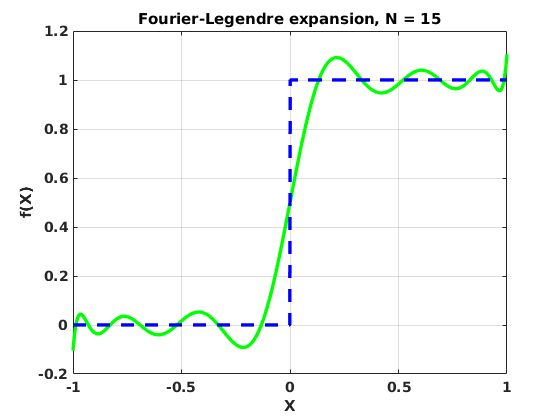
\includegraphics{lec20_ex.png}
\caption{Fourier-Legendre expansion with $N=15$.}
\label{fig:lec20-ex}
\end{marginfigure}

\begin{marginfigure}
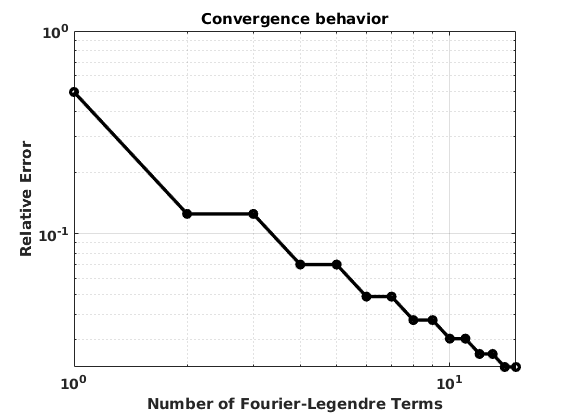
\includegraphics{lec20_converge.png}
\caption{Convergence of Fourier-Legendre expansion}
\label{fig:lec20-conv}
\end{marginfigure}
\newthought{A plot of} the Fourier-Legendre expansion is shown in Figure \ref{fig:lec20-ex} and the convergence behavior is shown in Figure \ref{fig:lec20-conv}.  Several things should be noted.
\begin{enumerate}
\item Clearly we can see from Figure \ref{fig:lec20-ex} that the Fourier-Legendre expansion is converging to the average value at the point of discontinuity at $x=0$.  
\item Like other Fourier expansions, perturbations (``wiggliness'') is introduced by that discontinuity and this is something that we should learn to expect.
\item Also note that from Figure \ref{fig:lec20-conv} we see that the expansion improves when we add the $c_0$ term, the $c_1$ term, $c_3$ term, and all odd-numbered terms but the relative error does not change for the even-numbered terms $c_2,c_4,\dots,c_{14}$.  Looking at $f(x)$ is should be apparent that, in some sense anyway, the function is \emph{odd}---or at least ``odd-ish''; you could make it odd by subtracting out a constant term (i.e. $f(x) - 0.5$ is odd and the $c_0$ coefficient is equal to that 0.5). The even-order Legendre polynomials are even and orthogonal to $f(x)$.  
\end{enumerate}
